En este capítulo se  el modelo de información del sistema, en el que podrá encontrar las diferentes entidades que son de interés dentro del sistema, estas entidades son cualquier concepto del que se requiera llevar registro, estas entidades pueden ser:

    \begin{bGlosario}
        \bTerm{tPersonas}{Personas} Tales como cliente, profesor, alumno, etc.
        \bTerm{tEventos}{Eventos}   Tales como compra, venta, inscipción, cita, etc
        \bTerm{tObjetos}{Objetos}   Tales como producto, mueble, etc.
        \bTerm{tLugar}{Lugar}       Ciudad, Pais,etc.
        \bTerm{tConcepto}{Concepto} Cuenta, curso, etc.
    \end{bGlosario}

Cada dato que nos interese de una entidad se coloca en forma de atributo, acompañado de su respectiva descripción y tipo de dato. Con ello, se busca indicar la naturaleza del atributo y restringir sus valores posibles. Entre los tipos de dato más comunes, encontramos los siguientes:

    \begin{bGlosario}

	    \bTerm{tBool}{bool}
	    Valor booleano, es decir, toma únicamente los valores 0 y 1.

        \bTerm{tInt}{int}
            Solo valores enteros, incluido el 0
            
        \bTerm{tNumeric}{numeric} (precisión, escala)
            Número cuyo número de dígitos está indicado por precisión, de los cuales
            los definidos en escala son a la izquierda del punto y el resto a la derecha.
            
        \bTerm{tChar}{Char}
            Cadena de caracteres de la longitud indicada, si se guarda una cadena de menor
            tamaño, los caracteres no utilizados serán espacios en blanco, por ejemplo si
            se ingresó el texto ‘edgar’ en un atributo de longitud 50, además de sus 5 caracteres
            tendrá 45 espacios en blanco al final, así su longitud siempre será 50.
            
        \bTerm{tVarchar}{varchar} (longitud)
            Cadena de caracteres de longitud variable. Por ejemplo, si se ingresa el texto 'edgar'
            en un atributo de longitud 50, entonces tendrá solo 5 caracteres.
            
        \bTerm{tDate}{date} Fecha
        \bTerm{tTime}{time} Hora
        \bTerm{tTimestamp}{timestamp} Fecha y hora
        \bTerm{tMoney}{money} Unidades monetarias en moneda nacional
        \bTerm{tEmail}{E-mail}
    
        Solo valores enteros, incluido el 0
    \end{bGlosario}

Cada dato puede tener restricciones adicionales, entre las que se encuentran:
    
    \begin{bGlosario}
    
        \bTerm{tRequerido}{Requerido}
            Indica que el dato es obligatorio y no puede existir un registro sin que éste tenga
            un valor.
            
        \bTerm{tUnico}{Único}
            Indica que los valores para un atributo o combinación de estos no se deben
            repetir en los diferentes registros.
            
        \bTerm{tDefault}{default}
            Permite especificar un valor por defecto para el atributo.
            
        \bTerm{tPrimaryKey}{primary key}
            Indica el atributo o combinación de éstos que serán la llave primaria. La llave
            primaria es el identificador único de cada registro dentro de la tabla, por lo
            que debe ser requerido y único.
            
        \bTerm{tForeignKey}{Foreign key}
            Indica el atributo o conjunto de éstos que son llave foránea y apuntan a otra
            tabla, esto es, sus valores posibles solo pueden ser aquellos que existan en la
            llave primaria a la que apuntan. FK(Tabla.atributo).
            
        \bTerm{tCHECK}{CHECK} (condicionACumplir)
            Indica que se debe cumplir una condición sobre un atributo en particular para
            que se permita el registro o actualización de datos.
            
        \bTerm{tRango}{Rango} [LimiteInf, LimiteSuperior]
            Indica que los valores posibles deben estar dentro de ese rango.
            
        \bTerm{tNumCaracteres}{NumCaracteres}[NumInf, NumSup]
            Indica que el número de caracteres debe estar en el rango especificado.
            
        \bTerm{tExpresionRegular}{ExpresionRegular} (expresion)
            Indica que se debe de cumplir con la expresión indicada.

        \bTerm{talfanum}{Caracteres alfanuméricos} 
            Es el conjunto de caracteres numéricos y alfabéticos.

        \bTerm{tcespecia}{Caracteres especiales} 
            El sistema puede aceptar los siquientes caracteres: \$ , \& , \# , \% , \_ , \~ , entre otros.

            
    \end{bGlosario}
    
\clearpage

\section{Diagrama de base de datos}

\begin{figure}[hbtp!]
    \begin{center}
           % \includegraphics[width=.65\textwidth]{negocio/images/MI-POA-CH}
            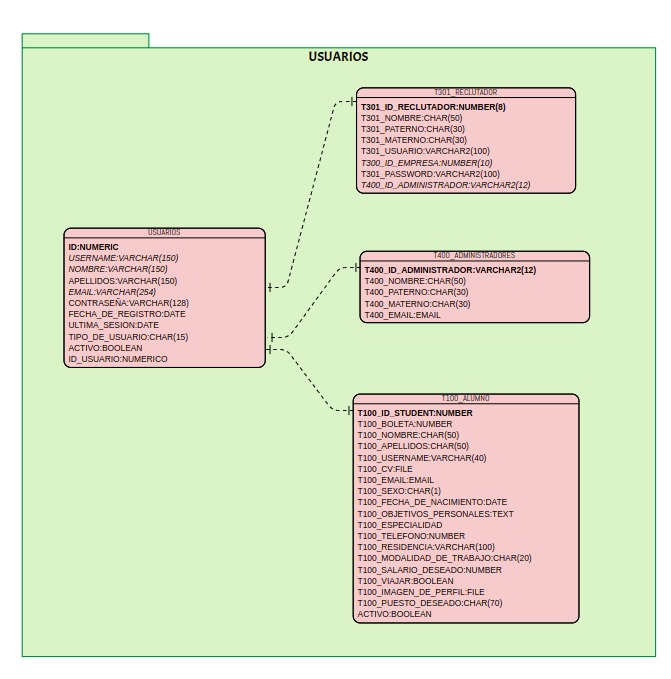
\includegraphics[width=.6\textwidth]{anexos/imagenes/Usuarios.jpeg}
            
    \end{center}
        \label{fig:MI-Planeacion}
            \caption{Diagrama de base de datos del módulo de Usuarios}
    
    \end{figure}

% En la figura  \ref{fig:MI-PlaneacionI}
%\begin{figure}[hbtp!]
%    \begin{center}
%        \includegraphics[width=.7\textwidth]{negocio/images/MI-POA-CAT}
%    \end{center}
%    \label{fig:MI-PlaneacionI}
%\end{figure}
%
%\begin{figure}[hbtp!]
%    \begin{center}
%        \includegraphics[width=.7\textwidth]{negocio/images/MI-POA-CFG}
%    \end{center}
%    \label{fig:MI-PlaneacionII}
%\end{figure}
%
%\begin{figure}[hbtp!]
%    \begin{center}
%        \includegraphics[width=.7\textwidth]{negocio/images/MI-POA-PLA}
%    \end{center}
%    \label{fig:MI-PlaneacionIII}
%\end{figure}

%---------------------Usuario-----------------------------
\begin{cdtEntidad}{users}{Usuario}{
        Esta entidad es generada por Django. 
    }
	    \brAttr{id}{Id de usuario}{tInt}{
	        Identificador único para cada registro de la entidad usuarios.
            Restricciones adicionales:
            \begin{Citemize}
                \item \refElem{tPrimaryKey}
                \item \refElem{tUnico}
            \end{Citemize}
        }{\datRequerido}

        \brAttr{nombre}{Nombre}{tVarchar}{
	        Es el nombre de la persona con el cual se registra dentro del sistema.
        }{\datRequerido}

        \brAttr{email}{Correo electrónico}{tEmail}{
	        Es el correo del alumno con el cual se identificara como unico dentro del sistema.
	        Restricciones adicionales:
            \begin{Citemize}
                \item \refElem{tUnico}
            \end{Citemize}
        }{\datRequerido}
    
        \brAttr{password}{Contraseña}{tVarchar}{
	        Es la contraseña de acceso al sistema para el usuario.
            Restricciones adicionales:
            \begin{Citemize}
                \item Debe de cumplir con el formato correcto de acuerdo a \refIdElem{RN-N006}
            \end{Citemize}
        }{\datRequerido}

        \brAttr{fecharegis}{Fecha de registro}{tDate}{
	        Es la fecha en la que el usuario crea su cuenta en el sistema y el propio sistema 
            la registra.
        }{\datRequerido}

        \brAttr{ultsesion}{Ultima sesión}{tDate}{
	        Es la fecha en la que el usuario inició sesión en el sistema (se registra automáticamente).
        }{\datRequerido}

        \brAttr{idtipo}{Id de tipo}{tNumeric}{
            Es la referencia a la entidad \refElem{users}
            Restricciones adicionales:
            \begin{Citemize}
                \item \refElem{tForeignKey}
                \item \refElem{tUnico}
            \end{Citemize}
        }{\datRequerido}

        \brAttr{status}{Activo}{tBool}{
	        Es el estado de la cuenta del usuario dentro del sistema.
        }{\datRequerido}
\end{cdtEntidad}

%---------------------Empresa-----------------------------
\begin{cdtEntidad}{empresa}{Empresa}{
    Empresa constituida que publica vacantes en el sistema siempre y cuando lo haya permitido el 
    encargado/colaborador del sistema.
    }

    \brAttr{id}{Id de la empresa}{tInt}{
	    Identificador único para cada registro de la empresa.
        Restricciones adicionales:
        \begin{Citemize}
            \item \refElem{tPrimaryKey}
            \item \refElem{tUnico}
        \end{Citemize}
    }{\datRequerido} 

    \brAttr{nombre}{Nombre}{tVarchar}{
        Nombre de la empresa con el que se registra en el sistema.
    }{\datRequerido}

    \brAttr{rfc}{RFC}{tVarchar}{
        RFC de la empresa.
        Restricciones adicionales:
        \begin{Citemize}
            \item Debe de cumplir con la regla de negocio ...
            \item \refElem{tUnico}
        \end{Citemize}
    }{\datRequerido}

    \brAttr{razonsocial}{Razón social}{tVarchar}{
        Razon social de la empresa.
    }{\datRequerido}

    \brAttr{pageweb}{Página Web}{tVarchar}{
        Es el URL de la oágina de la empresa.
    }{\datOpcional}

    %\brAttr{mision}{Misión}{tVarchar}{Descripción}{\datOpcional}
    %\brAttr{vision}{Vision}{tVarchar}{Descripción}{\datOpcional}
    %\brAttr{fecha-alta}{Fecha de alta}{tDate}{Descripción}{\datOpcional}
    %\brAttr{id-admin}{Id del administrador}{tVarchar}{
	   %     Es el correo del alumno con el cual se identificara como unico dentro del sistema.
	   %     Restricciones adicionales:
     %       \begin{Citemize}
      %          \item \refElem{tForeignKey}
      %          \item \refElem{tUnico}
      %      \end{Citemize}
      %  }{\datRequerido}
\end{cdtEntidad}

%---------------------Reclutador-----------------------------
\begin{cdtEntidad}{reclutador}{Reclutador}{
    Es el personal de recursos humanos de la empresa que ya esta registrada en el sistema.}
    \brAttr{id}{Id de reclutador}{tInt}{
        Identificador único para cada registro de un reclutador.
        Restricciones adicionales:
        \begin{Citemize}
            \item \refElem{tPrimaryKey}
            \item \refElem{tUnico}
        \end{Citemize}
    }{\datRequerido} 

    \brAttr{nombre}{Nombre}{tChar}{
        Nombre del reclutador con el cual se registra en el sistema.
        Restricciones adicionales:
            \begin{Citemize}
                \item No debe de execer de 50 caracteres.
            \end{Citemize}
    }{\datRequerido}

    \brAttr{papellido}{Primer apellido}{tChar}{
        Primer apellido del reclutador con el cual se registra en el sistema.
        Restricciones adicionales:
            \begin{Citemize}
                \item No debe de execer de 60 caracteres.
            \end{Citemize}
    }{\datRequerido}

    \brAttr{sapellido}{Segundo apellido}{tChar}{
        Segundo apellido del reclutador con el cual se registra en el sistema.
        Restricciones adicionales:
            \begin{Citemize}
                \item No debe de execer de 60 caracteres.
            \end{Citemize}
    }{\datOpcional}

    \brAttr{telefono}{Telefono}{tNumeric}{
        Número del telefono del reclutador.
        Restricciones adicionales:
            \begin{Citemize}
                \item Tiene que ser exactamente de 10 dígitos.
            \end{Citemize}
    }{\datRequerido}

    \brAttr{email}{Correo electrónico}{tEmail}{
	    Es el correo del reclutador.
	    Restricciones adicionales:
            \begin{Citemize}
                \item \refElem{tUnico}
            \end{Citemize}
    }{\datRequerido}

    \brAttr{id-impresa}{Id}{tInt}{
        Es la referencia al id del registro de la empresa.
        Restricciones adicionales:
        \begin{Citemize}
            \item \refElem{tForeignKey}
        \end{Citemize}
    
    }{\datOpcional}
    %\brAttr{id-admin}{Id}{tInt}{Descripción}{\datOpcional}
\end{cdtEntidad}
%---------------------Alumno-----------------------------
\begin{cdtEntidad}{estudiante}{Alumno}{desc}
    Un alumno es un tipo de usuario dentro del sistema 
    \brAttr{id-alumno}{Id}{tInt}{
        Identificador único para cada registro de la entidad alumno.
            Restricciones adicionales:
            \begin{Citemize}
                \item \refElem{tPrimaryKey}
                \item \refElem{tUnico}
            \end{Citemize}
    }{\datRequerido} 

    \brAttr{boleta}{Número de boleta}{tNumeric}{
        Es el número de boleta de los alumnos del Instituto Politécnico Nacional.
            Restricciones adicionales:
            \begin{Citemize}
                \item Debe de cumplir con la regla de negocio ...
                \item \refElem{tUnico}
            \end{Citemize}
    }{\datOpcional}

    \brAttr{nombre}{Nombre}{tChar}{
        Nombre del alumno con el cual se registra en el sistema.
        Restricciones adicionales:
            \begin{Citemize}
                \item No debe de execer de 50 caracteres.
            \end{Citemize}
    }{\datRequerido}

    \brAttr{papellido}{Primer apellido}{tChar}{
        Primer apellido del alumno con el cual se registra en el sistema.
        Restricciones adicionales:
            \begin{Citemize}
                \item No debe de execer de 60 caracteres.
            \end{Citemize}
    }{\datRequerido}

    \brAttr{sapellido}{Segundo apellido}{tChar}{
        Segundo apellido del alumno con el cual se registra en el sistema.
        Restricciones adicionales:
            \begin{Citemize}
                \item No debe de execer de 60 caracteres.
            \end{Citemize}
    }{\datOpcional}

    \brAttr{pdfcv}{CV/Resume}{tVarchar}{
        Archivo en formato \textbf{.pdf} del alumno.
        Restricciones adicionales:
            \begin{Citemize}
                \item No debe de execer de 100 caracteres.
            \end{Citemize}
    }{\datOpcional}

    \brAttr{email}{Correo electrónico}{tEmail}{
	    Es el correo del alumno.
	    Restricciones adicionales:
            \begin{Citemize}
                \item \refElem{tUnico}
            \end{Citemize}
    }{\datRequerido}
    
    \brAttr{objetivospersonales}{Objetivos personales}{tVarchar}{
        Descripción de los objetivos personales del alumno.
    }{\datOpcional}
    
    \brAttr{puestodeseado}{Puesto deseado}{tChar}{
        Nombre del puesto deseado del alumno.
        Restricciones adicionales:
            \begin{Citemize}
                \item No debe de execer de 70 caracteres.
            \end{Citemize}
    }{\datOpcional}
    
    \brAttr{telefono}{Telefono}{tNumeric}{
        Número del telefono del alumno.
        Restricciones adicionales:
            \begin{Citemize}
                \item Tiene que ser exactamente de 10 dígitos.
            \end{Citemize}
    }{\datRequerido}
    
    \brAttr{recidencia}{Recidencia}{tVarchar}{
        Lugar donde se ubica el alumno.
    }{\datRequerido}

    \brAttr{salario}{Salario deseado}{tNumeric}{
        Cantidad salarial que desea percibir el alumno.
    }{\datOpcional}

    \brAttr{reubicable}{Reubicable}{tBool}{
        Indica si el alumno esta dispuesto a cambiar de lugar de recidencia o no.
    }{\datOpcional}

    \brAttr{imagenperfil}{Imagen de perfil}{tVarchar}{
        Es la imagen del perfil del alumno:
        Los tipos de archivos que se permiten son:
            \begin{Citemize}
                \item .png
                \item .jpg
                \item .jpge
            \end{Citemize}
    }{\datOpcional}

    \brAttr{status}{Activo}{tBool}{
	        Es el estado de la cuenta del usuario dentro del sistema.
    }{\datOpcional}
   
    \brAttr{modalidad}{Tipo de trabajo}{tVarchar}{
       Es el tipo de trabajo que prefiere el alumno.
       Los valores posibles son:
            \begin{Citemize}
                \item Hibrido
                \item Presencial
                \item Home oficce
            \end{Citemize}
    }{\datOpcional}

\end{cdtEntidad}

%---------------------Historial Academico-----------------------------
\begin{cdtEntidad}{hacademico}{Historial Academico}{desc}
    \brAttr{id-vacante}{Id}{tInt}{Descripción}{\datRequerido} 
    \brAttr{intitucion}{Institucion}{tVarchar}{Descripción}{\datRequerido}
    \brAttr{carrera}{Carrera}{tVarchar}{Descripción}{\datRequerido}
    \brAttr{inicio}{Fecha de inicio}{tVarchar}{Descripción}{\datRequerido}
    \brAttr{fin}{Fecha final}{tVarchar}{Descripción}{\datRequerido}
    
\end{cdtEntidad}

%---------------------Habilidades----------------------------
\begin{cdtEntidad}{habilidad}{Catalogo Habilidades}{desc}
    \brAttr{id-habilidad}{Id}{tInt}{Descripción}{\datRequerido} 
    \brAttr{descripcion}{Carrera}{tVarchar}{Descripción}{\datRequerido}
    \brAttr{tipo}{Fecha de inicio}{tVarchar}{Descripción}{\datRequerido}
\end{cdtEntidad}


%---------------------Vacante----------------------------
\begin{cdtEntidad}{vacante}{Vacante}{
    Vacante publicada por un reclutador de una empresa.
}
    \brAttr{id}{Id}{tInt}{Descripción}{\datRequerido} 
    \brAttr{titulo}{Titulo}{tVarchar}{Descripción}{\datRequerido}
    \brAttr{descripcion}{Fecha de inicio}{tVarchar}{Descripción}{\datRequerido}
    \brAttr{salario-min}{Salario mínimo}{tVarchar}{Descripción}{\datRequerido}
    \brAttr{saralio-max}{Salario maximo}{tVarchar}{Descripción}{\datRequerido}
    \brAttr{ubicacion}{Salario maximo}{tVarchar}{Descripción}{\datRequerido}
\end{cdtEntidad}

